%background
\chapter{Simulated Environment} 

% 

In order for autonomous vehicles to operate safely in the real world, they must be able to adapt to a multitude of changing conditions. Before fully self-driving vehicles hit the road, they undergo a lengthy period of testing where the vehicle's sensors and artificial intelligence are tested in a variety of simulated real-world environments. Simulation has become the backbone of the autonomous driving industry, providing a means to collect extensive amounts of data for model training as well as providing a safe testbed to crash-test these models. In this chapter, we would like to create a simulator for training autonomous diving algorithms.

A simplified highway environment would be created to train deep learning models for the autonomous vehicle to gain better decision making ability of speed control and  lane changing.

The simulated environment is constructed based on ROS and Gazebo and the Reinforcement Learning Algorithms are implemented by OpenAI-Gym. An open source car model kit, Drive-by-Wire (DBW) Kit, is adopted to play the role of the autonomous vehicle. An overall architecture of the simulation environment is shown as Fig. \ref{fig:sim-env}.

\begin{figure}[h]
\centering
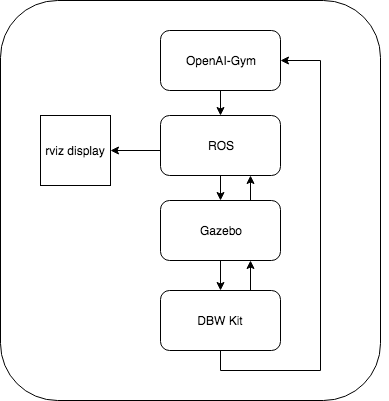
\includegraphics[width=0.7\textwidth]{figs/ch2/simulation-architecture}
\caption{Architecture of the simulation environment.}
\label{fig:sim-env}.
\end{figure}

% why openai-gym

OpenAI was founded in late 2015 as a non-profit with a mission to "build safe artificial general intelligence (AGI) and ensure AGI's benefits are as widely and evenly distributed as possible." In addition to exploring many issues regarding AGI, one major contribution that OpenAI made to the machine learning world was developing both the Gym and Universe software platforms. OpenAI-Gym is a collection of environments / problems designed for testing and developing reinforcement learning algorithms --- it saves the user from having to create complicated environments. Gym is written in Python, and there are multiple environments such as robot simulations or Atari games. There is also an online leaderboard for people to compare results and code.

% why ros

% why gazebo

The usual basic requirements to robot simulators are an accurate physics simulation (such as object velocity, inertia, friction, position and orientation, etc.), high quality rendering (for shape, dimensions, colors, and texture of objects), integration with the Robot Operating System (ROS) framework and multi-platform performability. It provides great opportunities for modeling robots and their sensors together with developing robot control algorithms, realizing mobile robot simulation, visualization, locomotion and navigation in a realistic 3D environment. As mentioned in the paper \cite{jmeSim2012}, the high graphical fidelity in a robot simulation is important because the sensory input to the robot perceptual algorithms comes from virtual sensors, which are also provided by the simulation. For example, virtual cameras use the simulator rendering engine to obtain their images. If images from a simulated camera have incorrect similarity to real camera ones, then it is not possible to use them for object recognition and localization.

To avoid such a sort of problems, we use the robust and high graphical quality robot simulator --- Gazebo, which is an open source robotic simulation package that closely integrated with ROS. Gazebo uses the open source OGRE rendering engine, which produces good graphics fidelity, although it also employs the Open Dynamics Engine (ODE), which is estimated as sufficiently slow physics engine \cite{jmeSim2012}.

%%%%%%%%%%%%%%%%%%%%%%%%%%%%%%%%%%
\section{ROS}

Writing software for robots is difficult, particularly as the scale and scope of robotics continues to grow. Different types of robots can have wildly varying hardware, making code reuse nontrivial. A wide variety of frameworks were created to liberate researchers and developers from those way beyond their interests. Among them, Robot Operating System (ROS) framework \cite{ROS2009}  gained more popularity because of its generality and expansibility. ROS was designed to meet a specific set of challenges encountered when developing large-scale service robots as part of the STAIR project \cite{STAIR2007} at Stanford University and the Personal Robots Program \cite{PR2008} at Willow Garage, but the resulting architecture is far more general than the service-robot and mobile-manipulation domains.

The philosophical goals of ROS can be summarized as:

\begin{itemize}
\item Peer-to-peer 
\item Tools-based 
\item Multi-lingual 
\item Thin
\item Free and Open-Source
\end{itemize}

\subsection{Implementation}

The fundamental concepts of the ROS implementation are nodes, messages, topics, and services.

Nodes are processes that perform computation. ROS is designed to be modular at a fine-grained scale: a system is typically comprised of many nodes. In this context, the term "node" is interchangable with "software module". Our use of the term "node" arises from visualizations of ROS-based systems at runtime: when many nodes are running, it is convenient to render the peer-to-peer communications as a graph, with processes as graph nodes and the peer-to-peer links as arcs.

Nodes communicate with each other by passing messages. A message is a strictly typed data structure. Standard primitive types (integer, floating point, boolean, etc.) are supported, as are arrays of primitive types and constants. Messages can be composed of other messages, and arrays of other messages, nested arbitrarily deep.

A node sends a message by publishing it to a given topic, which is simply a string such as "odometry" or "map". A node that is interested in a certain kind of data will subscribe to the appropriate topic. There may be multiple concurrent publishers and subscribers for a single topic, and a single node may publish and/or subscribe to multiple topics. In general, publishers and subscribers are not aware of each others' existence.

\begin{figure}[h]
\centering
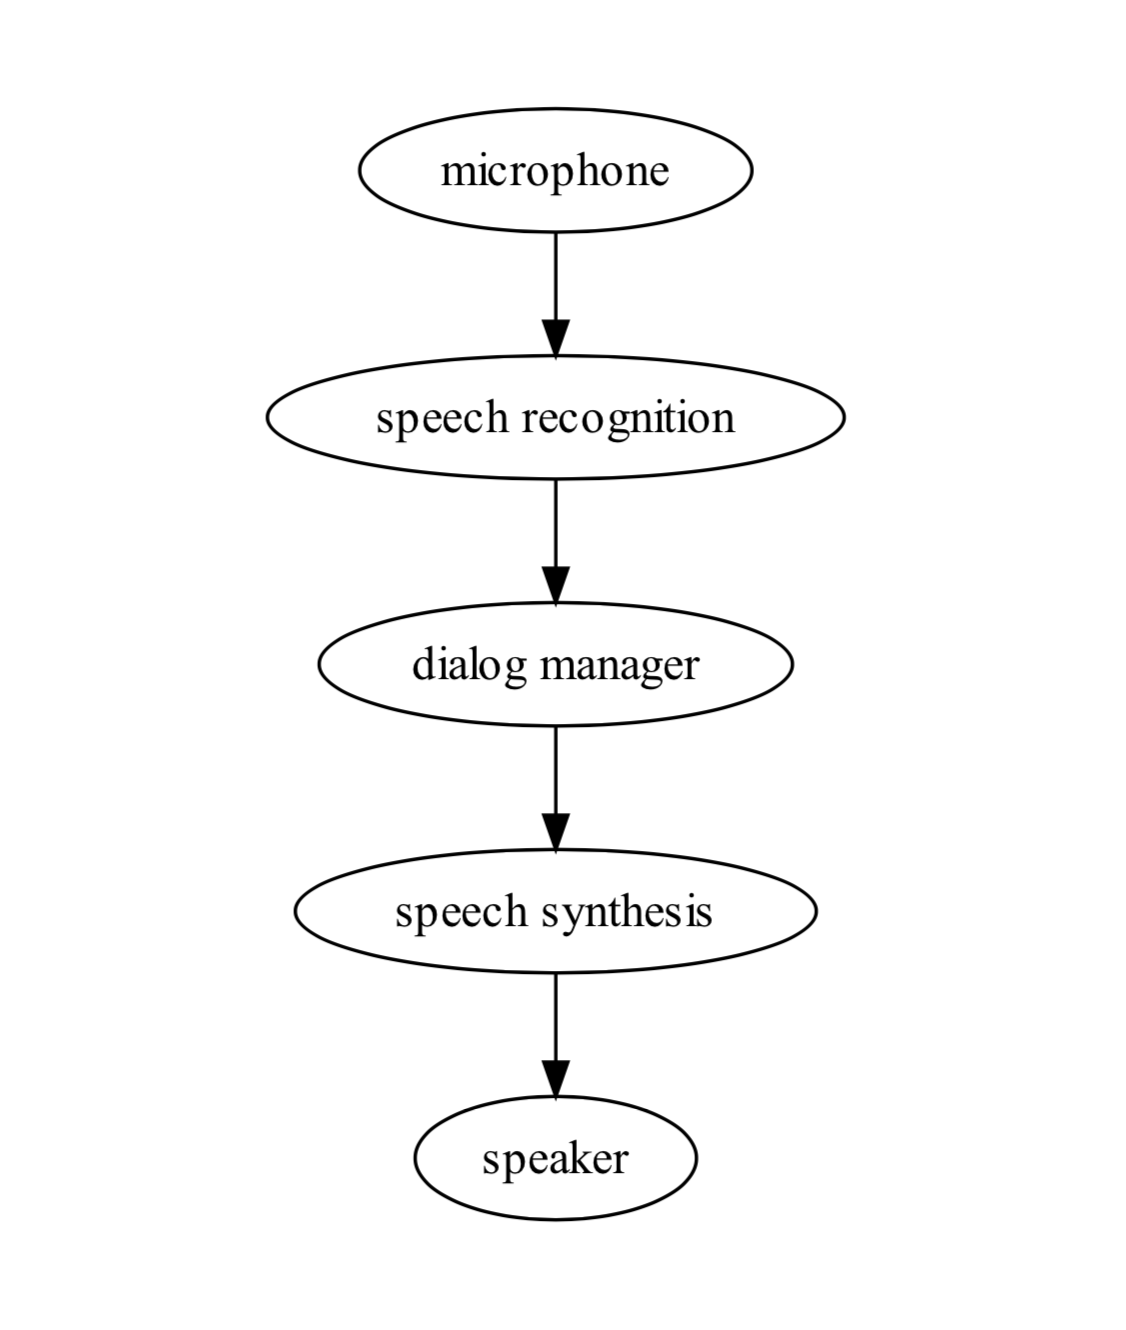
\includegraphics[width=0.6\textwidth]{figs/ch2/ros-pipeline}
\caption{Communication pipeline.}
\end{figure}

\subsection{Collaborative Development}

Due to the vast scope of robotics and artificial intelligence, collaboration between modules is necessary in order to build large systems. To support collaborative development, the ROS software system is organized into packages. Our definition of "package" is deliberately open-ended: a ROS package is simply a directory which contains an XML file describing the package and stating any dependencies.

A collection of ROS packages is a directory tree with ROS packages at the leaves: a ROS package repository may thus contain an arbitrarily complex scheme of subdirectories. For example, one ROS repository has root directories including "nav", "vision" and "motion planning" each of which contains many packages as subdirectories.

The open-ended nature of ROS packages allows for great variation in their structure and purpose: some ROS packages wrap existing software, such as Player or OpenCV, automating their builds and exporting their functionality. Some packages build nodes for use in ROS graphs, other packages provide libraries and standalone executables, and still others provide scripts to automate demonstrations and tests. The packaging system is meant to partition the building of ROS-based software into small, manageable chunks, each of which can be maintained and developed on its own schedule by its own team of developers.

\subsection{Visualization and Monitoring}

While designing and debugging robotics software, it often becomes necessary to observe some state while the system is running. Although \textit{printf} is a familiar technique for debugging programs on a single machine, this technique can be difficult to extend to large-scale distributed systems, and can become unwieldy for general-purpose monitoring.

Instead, ROS can exploit the dynamic nature of the connectivity graph to "tap into" any message stream on the system. Furthermore, the decoupling between publishers and subscribers allows for the creation of general-purpose visualizers. Simple programs can be written which subscribe to a particular topic name and plot a particular type of data, such as laser scans or images. However, a more powerful concept is a visualization program which uses a plugin architecture: this is done in the \textit{rviz} program, which is distributed with ROS. Visualization panels can be dynamically instantiated to view a large variety of datatypes, such as images, point clouds, geometric primitives (such as object recognition results), render robot poses and trajectories, etc. Plugins can be easily written to display more types of data.

A native ROS port is provided for Python, a dynamically-typed language supporting introspection. Using Python, a powerful utility called \textit{rostopic} was written to filter messages using expressions supplied on the command line, resulting in an instantly customizable "message tap" which can convert any portion of any data stream into a text stream. These text streams can be piped to other UNIX command-line tools such as \textit{grep}, \textit{sed}, and \textit{awk}, to create complex monitoring tools without writing any code.

Similarly, a tool called \textit{rxplot} provides the functionality of a virtual oscilloscope, plotting any variable in real-time as a time series, again through the use of Python introspection and expression evaluation.

\subsection{Transformations}

Robotic systems often need to track spatial relationships for a variety of reasons: between a mobile robot and some fixed frame of reference for localization, between the various sensor frames and manipulator frames, or to place frames on target objects for control purposes.

To simplify and unify the treatment of spatial frames, a transformation system has been written for ROS, called \textit{tf}. The \textit{tf} system constructs a dynamic transformation tree which relates all frames of reference in the system. As information streams in from the various subsystems of the robot (joint encoders, localization algorithms, etc.), the \textit{tf} system can produce streams of transformations between nodes on the tree by constructing a path between the desired nodes and performing the necessary calculations.

For example, the \textit{tf} system can be used to easily generate point clouds in a stationary "map" frame from laser scans received by a tilting laser scanner on a moving robot. As another example, consider a two-armed robot: the \textit{tf} system can stream the transformation from a wrist camera on one robotic arm to the moving tool tip of the second arm of the robot. These types of computations can be tedious, error- prone, and difficult to debug when coded by hand, but the \textit{tf} implementation, combined with the dynamic messaging infrastructure of ROS, allows for an automated, systematic approach.

%%%%%%%%%%%%%%%%%%%%%%%%%%%%%%%%%%
\section{Gazebo}

Gazebo is a 3D dynamic simulator with the ability to accurately and efficiently simulate populations of robots in complex indoor and outdoor environments, which makes it possible to rapidly test algorithms, design robots, perform regression testing, and train AI system using realistic scenarios. While similar to game engines, Gazebo offers physics simulation at a much higher degree of fidelity, a suite of sensors, and interfaces for both users and programs. Fig. \label{fig:pr2} gives a typical display of Gazebo and in the window is a PR2 robot \cite{PR2008} with its LIDAR sensor range displayed in blue.

\begin{figure}[h]
\centering
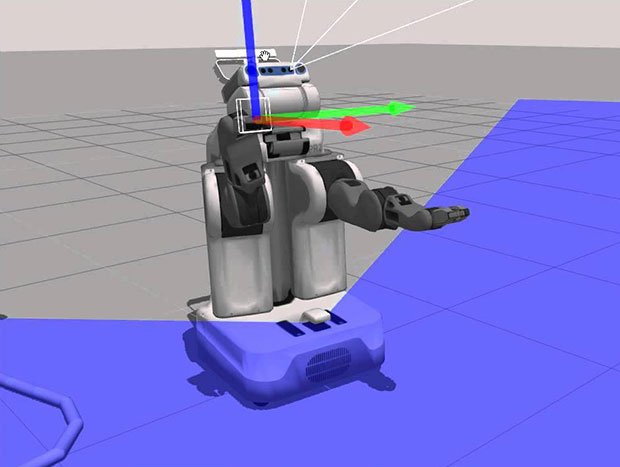
\includegraphics[width=0.8\textwidth]{figs/ch2/osrf.jpeg}
\caption{Gazebo for robot simulation.}
\label{fig:pr2}
\end{figure}

Typical uses of Gazebo include:

\begin{itemize}
\item testing robotics algorithms,
\item designing robots,
\item performing regression testing with realistic scenarios
\end{itemize}

A few key features of Gazebo include:

\begin{itemize}
\item multiple physics engines,
\item a rich library of robot models and environments,
\item a wide variety of sensors,
\item convenient programmatic and graphical interfaces
\end{itemize}

Gazebo is far from being the only choice for a 3D dynamics simulator. It is however one of the few that attempts to create realistic worlds for the robots rather than just human users. As more advanced sensors are developed and incorporated into Gazebo the line between simulation and reality will continue to blur, but accuracy in terms of robot sensors and actuators will remain an overriding goal.

\subsection{Architecture}

Gazebo's architecture has progressed through a couple iterations during which we learned how to best create a simple tool for both developers and end users. We realized from the start that a major feature of Gazebo should be the ability to easily create new robots, actuators, sensors, and arbitrary objects. As a result, Gazebo maintains a simple API for addition of these objects, which we term models, and the necessary hooks for interaction with client programs. A layer below this API resides the third party libraries that handle both the physics simulation and visualization. The particular libraries used were chosen based on their open source status, active user base, and maturity.

\begin{figure}[h]
\centering
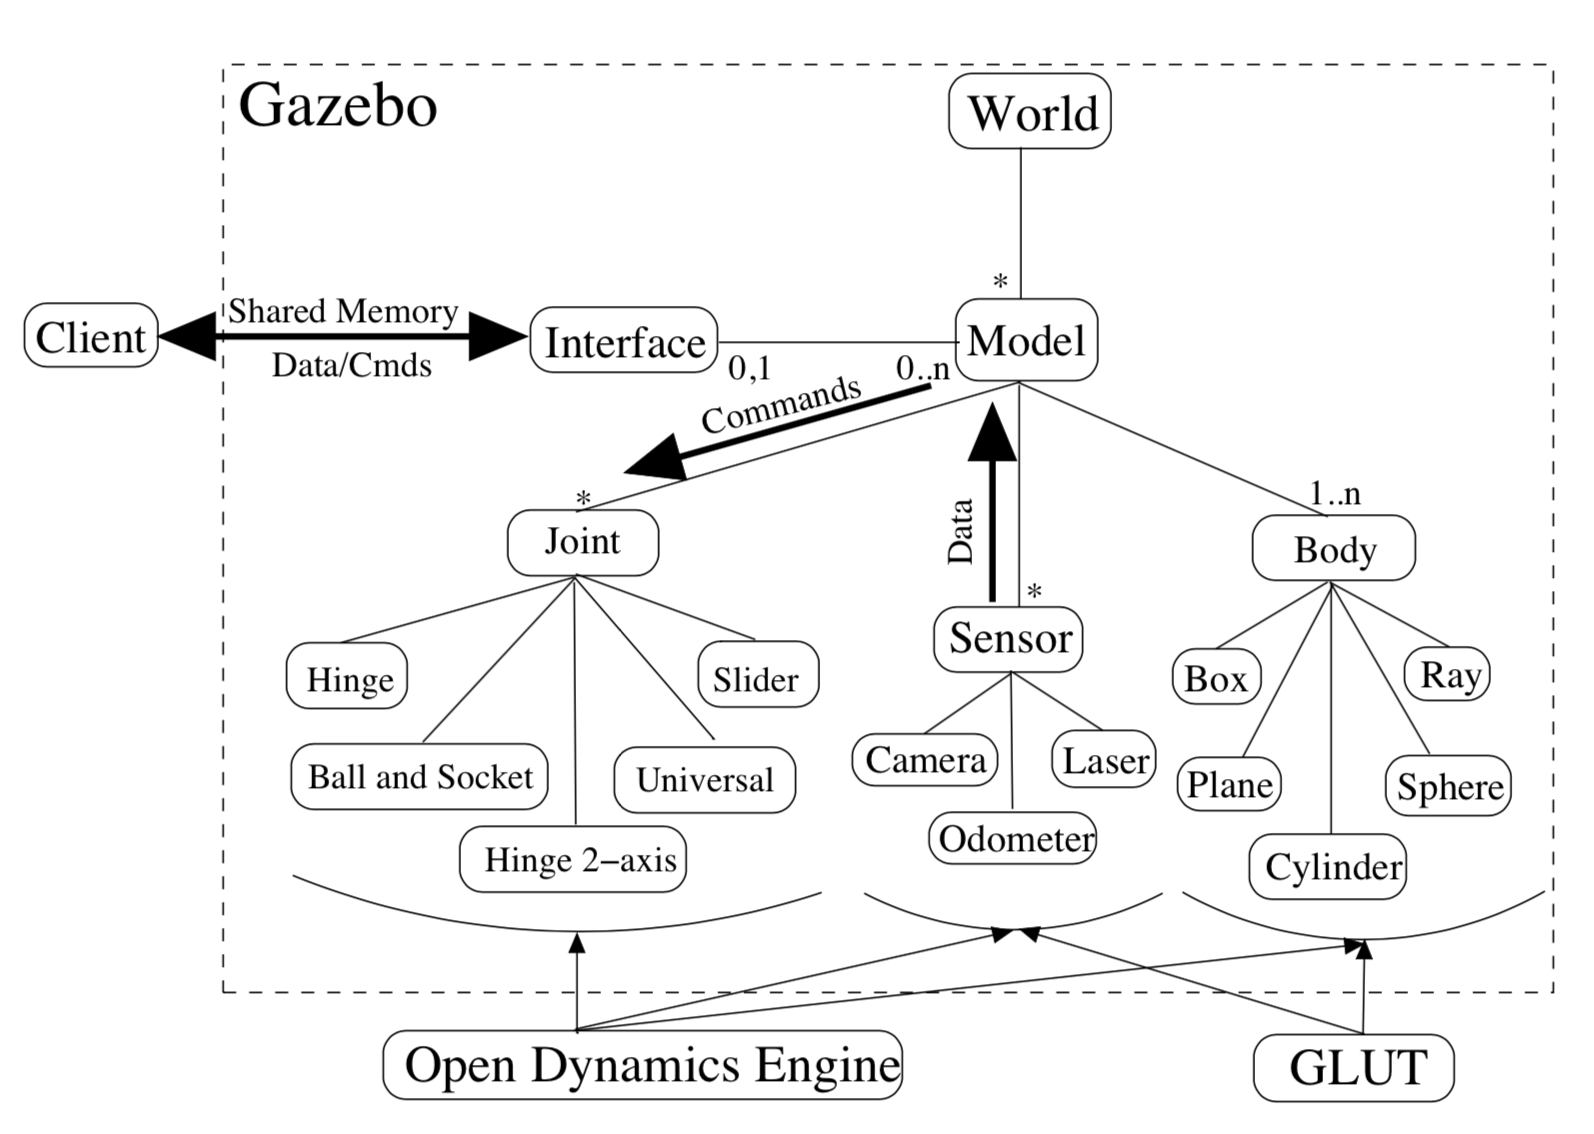
\includegraphics[width=0.8\textwidth]{figs/ch2/gazebo-structure}
\caption{Gazebo for robot simulation.}
\label{fig:gazebo-structure}
\end{figure}

This architecture is graphically depicted in Fig. \ref{fig:gazebo-structure}. The World represents the set of all models and environmental factors such as gravity and lighting. Each model is composed of at least one body and any number of joints and sensors. The third party libraries interface with Gazebo at the lowest level. This prevents models from becoming dependent on specific tools that may change in the future. Finally, client commands are received and data returned through a shared memory interface. A model can have many interfaces for functions involving, for example, control of joints and transmission of camera images.

\subsection{Physics Engine}

The Open Dynamics Engine, created by Russel Smith is a widely used physics engine in the open source community. It is designed to simulate the dynamics and kinematics associated with articulated rigid bodies. This engine includes many features such as numerous joints, collision detection, mass and rotational functions, and many geometries including arbitrary triangle meshes. Gazebo utilizes these features by providing a layer of abstraction situated between ODE and Gazebo models. This layer allows easy creation of both normal and abstract objects such as laser rays and ground planes while maintaining all the functionality provided by ODE. With this internal abstraction, it is possible to replace the underlying physics engine, should a better alternative become available.

\subsection{Visualization}

A well designed simulator usually provides some form of user interface, and Gazebo requires one that is both sophisticated and fast. The heart of Gazebo lies in its ability to simulate dynamics, and this requires significant work on behalf of the user's computer. A slow and cumbersome user interface would only detract from the simulator's primary purpose. To account for this, OpenGL and GLUT (OpenGL Utility Toolkit) were chosen as the default visualization tools.

OpenGL is a standard library for the creation of 2D and 3D interactive applications. It is platform independent, highly scalable, stable, and continually evolving. More importantly, many features in OpenGL have been implemented in graphic card hardware thereby freeing the CPU for other work such as the computationally expensive dynamics engine.

GLUT is a simple window system independent toolkit for OpenGL applications. Scenes rendered using OpenGL are displayed in windows created by GLUT. This toolkit also provides mechanisms for user interaction with Gazebo via standard input devices such as keyboards and mice. GLUT was chosen as the default windowing toolkit be- cause it is lightweight, easy to use, and platform independent.

\subsection{Customized Environment}

A complete environment is essentially a collection of models and sensors. The ground and buildings represent stationary models while robots and other objects are dynamic. Sensors remain separate from the dynamic simulation since they only collect data, or emit data if it is an active sensor.

\textbf{Models:} A model is any object that maintains a physical representation, which can be created by hand. The process starts with choosing the appropriate bodies and joints necessary to build an accurate model in both appearance and functionality. This encompasses anything from simple geometry to complex robots. Models are composed of at least one rigid body, zero or more joints and sensors, and interfaces to facilitate the flow of data.

Bodies represent the basic building blocks of a model. Their physical representation take the form of geometric shapes chosen from boxes, spheres, cylinders, planes, and lines. Each body has an assigned mass, friction, bounce factor, and rendering properties such as color, texture, transparency, etc.

Joints provide the mechanism to connect bodies together to form kinematic and dynamic relationships. A variety of joints are available including hinge joints for rotation along one or two axis, slider joints for translation along a single axis, ball and socket joints, and universal joints for rotation about two perpendicular joints. Besides connecting two bodies together, these joints can act like motors. When a force is applied to a joint, the friction between the connected body and other bodies cause motion. However, special care needs to be taken when connecting many joints in a single model as both the model and simulation can easily loose stability if incorrect parameters are chosen.

Interfaces provide the means by which client programs can access and control models. Commands sent over an interface can instruct a model to move joints, change the configuration of associated sensors, or request sensor data. The interfaces do not place restrictions on a model, thereby allowing the model to interpret the commands in anyway it sees fit.

\textbf{Sensors:} A robot can't perform useful tasks without sensors. A sensor in Gazebo is an abstract device lacking a physical representation. It only gains embodiment when incorporated into a model. This feature allows for the reuse of sensors in numerous models thereby reducing code and confusion.

There currently are three sensor implementations including an odometer, ray proximity, and a camera. Odometry is easily accessible through integration of the distance traveled. The ray proximity sensor returns the contact point of the closest object along the ray's path.

\textbf{External Interfaces:} From the users point of view, the models simulated in Gazebo are the same as their real counterparts, and are treated as a normal device capable of sending and receiving data. A second key advantage to this approach is that one can use abstract drivers inside a simulation. 

The low-level library provides a mechanism for any third-party robot device server interface with Gazebo. Going even further, a connection to the the library is not even necessary since Gazebo can be run independently for rapid model and sensor development. Currently the Gazebo library offers hooks to set wheel velocities, read data from a laser range finder, retrieve images from a camera, and insert simple objects into the environment at runtime. This data is communicated through shared memory for speed and efficiency.

\textbf{Environments:} Many environments in which robots operate are either well studied or carefully constructed. Deploying robots in a never before encountered world may cause unforeseen, and possibly negative, side effects. Lighting conditions, reflective surfaces, and odd objects can all play an effect on how a robot operates. A strategy of online testing can be extremely slow and tedious. Time can be spent much more productively by testing and modifying the robot controllers offline in preparation for the real experiments. The fine grained control of Gazebo, the ability to extrude 2D images into 3D structures, and terrain generation allow for the unique ability to hand create rough outlines of a new environment. 

As a result, the development time of the algorithms employed was greatly reduced. Gazebo made it possible to continue experimentation in the environment even after the physical robots were deployed. Elevation information collected by real sensors can be imported along with relevant structures to further blur the line between simulation and the real world. All of this culminates in the ability of Gazebo to reduce development and test time, and even allow experiments to virtually take place in almost any part of the world.

\subsection{Test Bed for Algorithm Design}

The design and implementation of new algorithms can be a difficult task that become particularly acute with the lack of convenient test environments. In situations such as this, Gazebo's sensory realism can play a time saving role. Traditionally, development of new algorithms either required custom simulators or direct testing on the hardware; Gazebo's realistic environments and simple interface can drastically reduce the turn around time from a conceptual stage to functional system.

%%%%%%%%%%%%%%%%%%%%%%%%%%%%%%%%%%
\section{OpenAI-Gym}

Reinforcement learning assumes that there is an agent that is situated in an environment. Each step, the agent takes an action, and it receives an observation and reward from the environment. An RL algorithm seeks to maximize some measure of the agent's total reward, as the agent interacts with the environment. In the RL literature, the environment is formalized as a partially observable Markov decision process (POMDP) \cite{Sutton1998RL}.

OpenAI Gym focuses on the episodic setting of reinforcement learning, where the agent's experience is broken down into a series of episodes. In each episode, the agent's initial state is randomly sampled from a distribution, and the interaction proceeds until the environment reaches a terminal state. The goal in episodic reinforcement learning is to maximize the expectation of total reward per episode, and to achieve a high level of performance in as few episodes as possible.

OpenAI Gym aims to combine the best elements of these previous benchmark collections, in a software package that is maximally convenient and accessible. It includes a diverse collection of Environments (POMDPs) with a common interface, and this collection will grow over time. The environments are versioned in a way that will ensure that results remain meaningful and reproducible as the software is updated.

\subsection{Design For Environment}

The design of OpenAI Gym is based on the experience developing and comparing reinforcement learning algorithms, and the experience using previous benchmark collections. Below, we will summarize some of our design decisions.

Two core concepts in Reinforcement Learning are the agent and the environment. OpenAi Gym's design focuses on providing an abstraction for the environment, but not for the agent. This choice was to maximize convenience for users and allow them to implement different styles of agent interface. First, one could imagine an ``online learning'' style, where the agent takes (observation, reward, done) as an input at each time-step and performs learning updates incrementally. In an alternative ``batch update'' style, a agent is called with observation as input, and the reward information is collected separately by the RL algorithm, and later it is used to compute an update. By only specifying the agent interface, it is allowed to write customized agents with either of these styles.

\subsection{Interfacing with ROS and Gazebo}

In the context of robotics, reinforcement learning offers a framework for the design of sophisticated and hard-to-engineer behaviors \cite{RLsurvey2013}. The challenge is to build a simple environment where this machine learning techniques can be validated, and later applied in a real scenario.

OpenAI Gym leaves interfaces to write customized agents, which makes it possible to integrate the Gym API with robotic hardware, validating reinforcement learning algorithms in real environments. Real-world operation is achieved combining Gazebo simulator with ROS.

\begin{figure}[h]
\centering
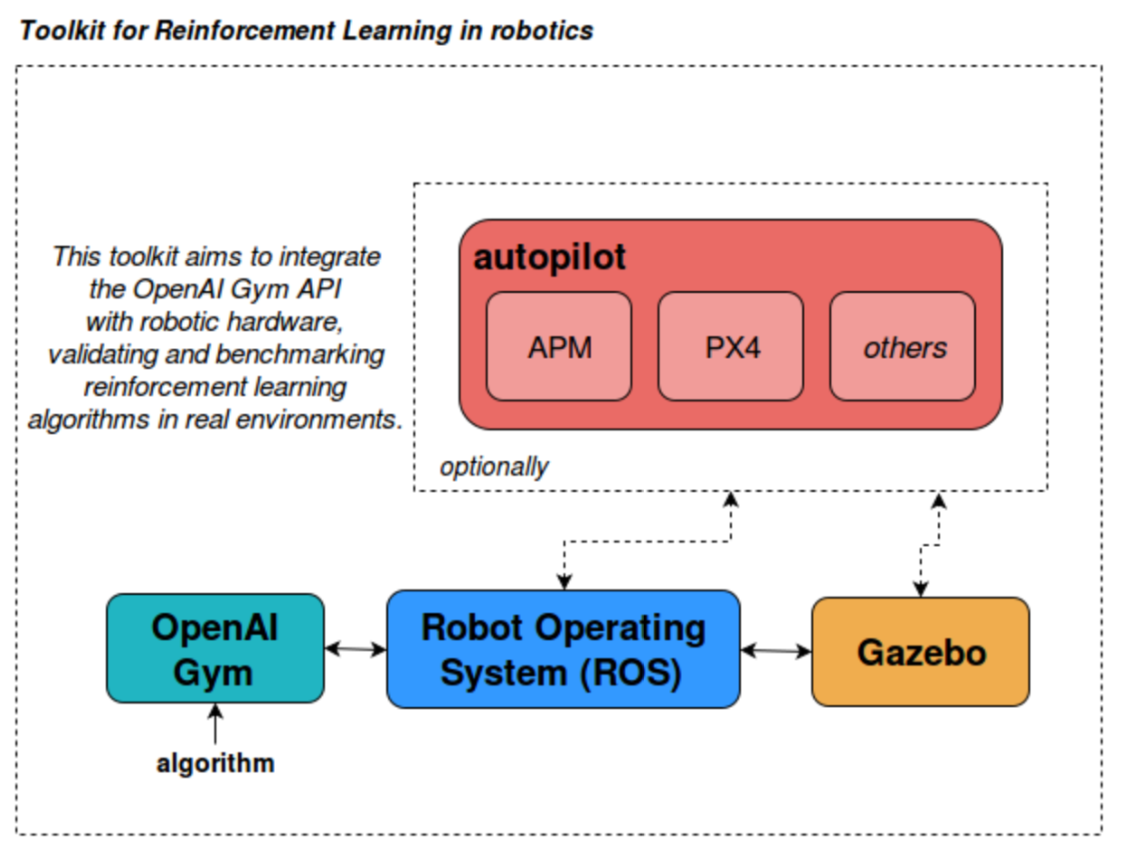
\includegraphics[width=0.8\textwidth]{figs/ch2/toolkit-of-openaigym}
\caption{Simplified software architecture used in OpenAI Gym for robotics.}
\label{fig:openai-archi}
\end{figure}

The architecture consists of three main software blocks: OpenAI Gym, ROS and Gazebo as shown in Fig. \ref{fig:openai-archi}. Environments developed in OpenAI Gym interact with ROS, which is the connection between the Gym itself and Gazebo simulator. Gazebo provides a robust physics engine, high-quality graphics, and convenient programmatic and graphical interfaces.

The physics engine needs a robot definition in order to simulate it, which is provided by ROS or a Gazebo plugin that interacts with an autopilot in some cases (depends on the robot software architecture).

\subsection{Example Use: Train a Cart-pole agent}

\begin{figure}[h]
\centering
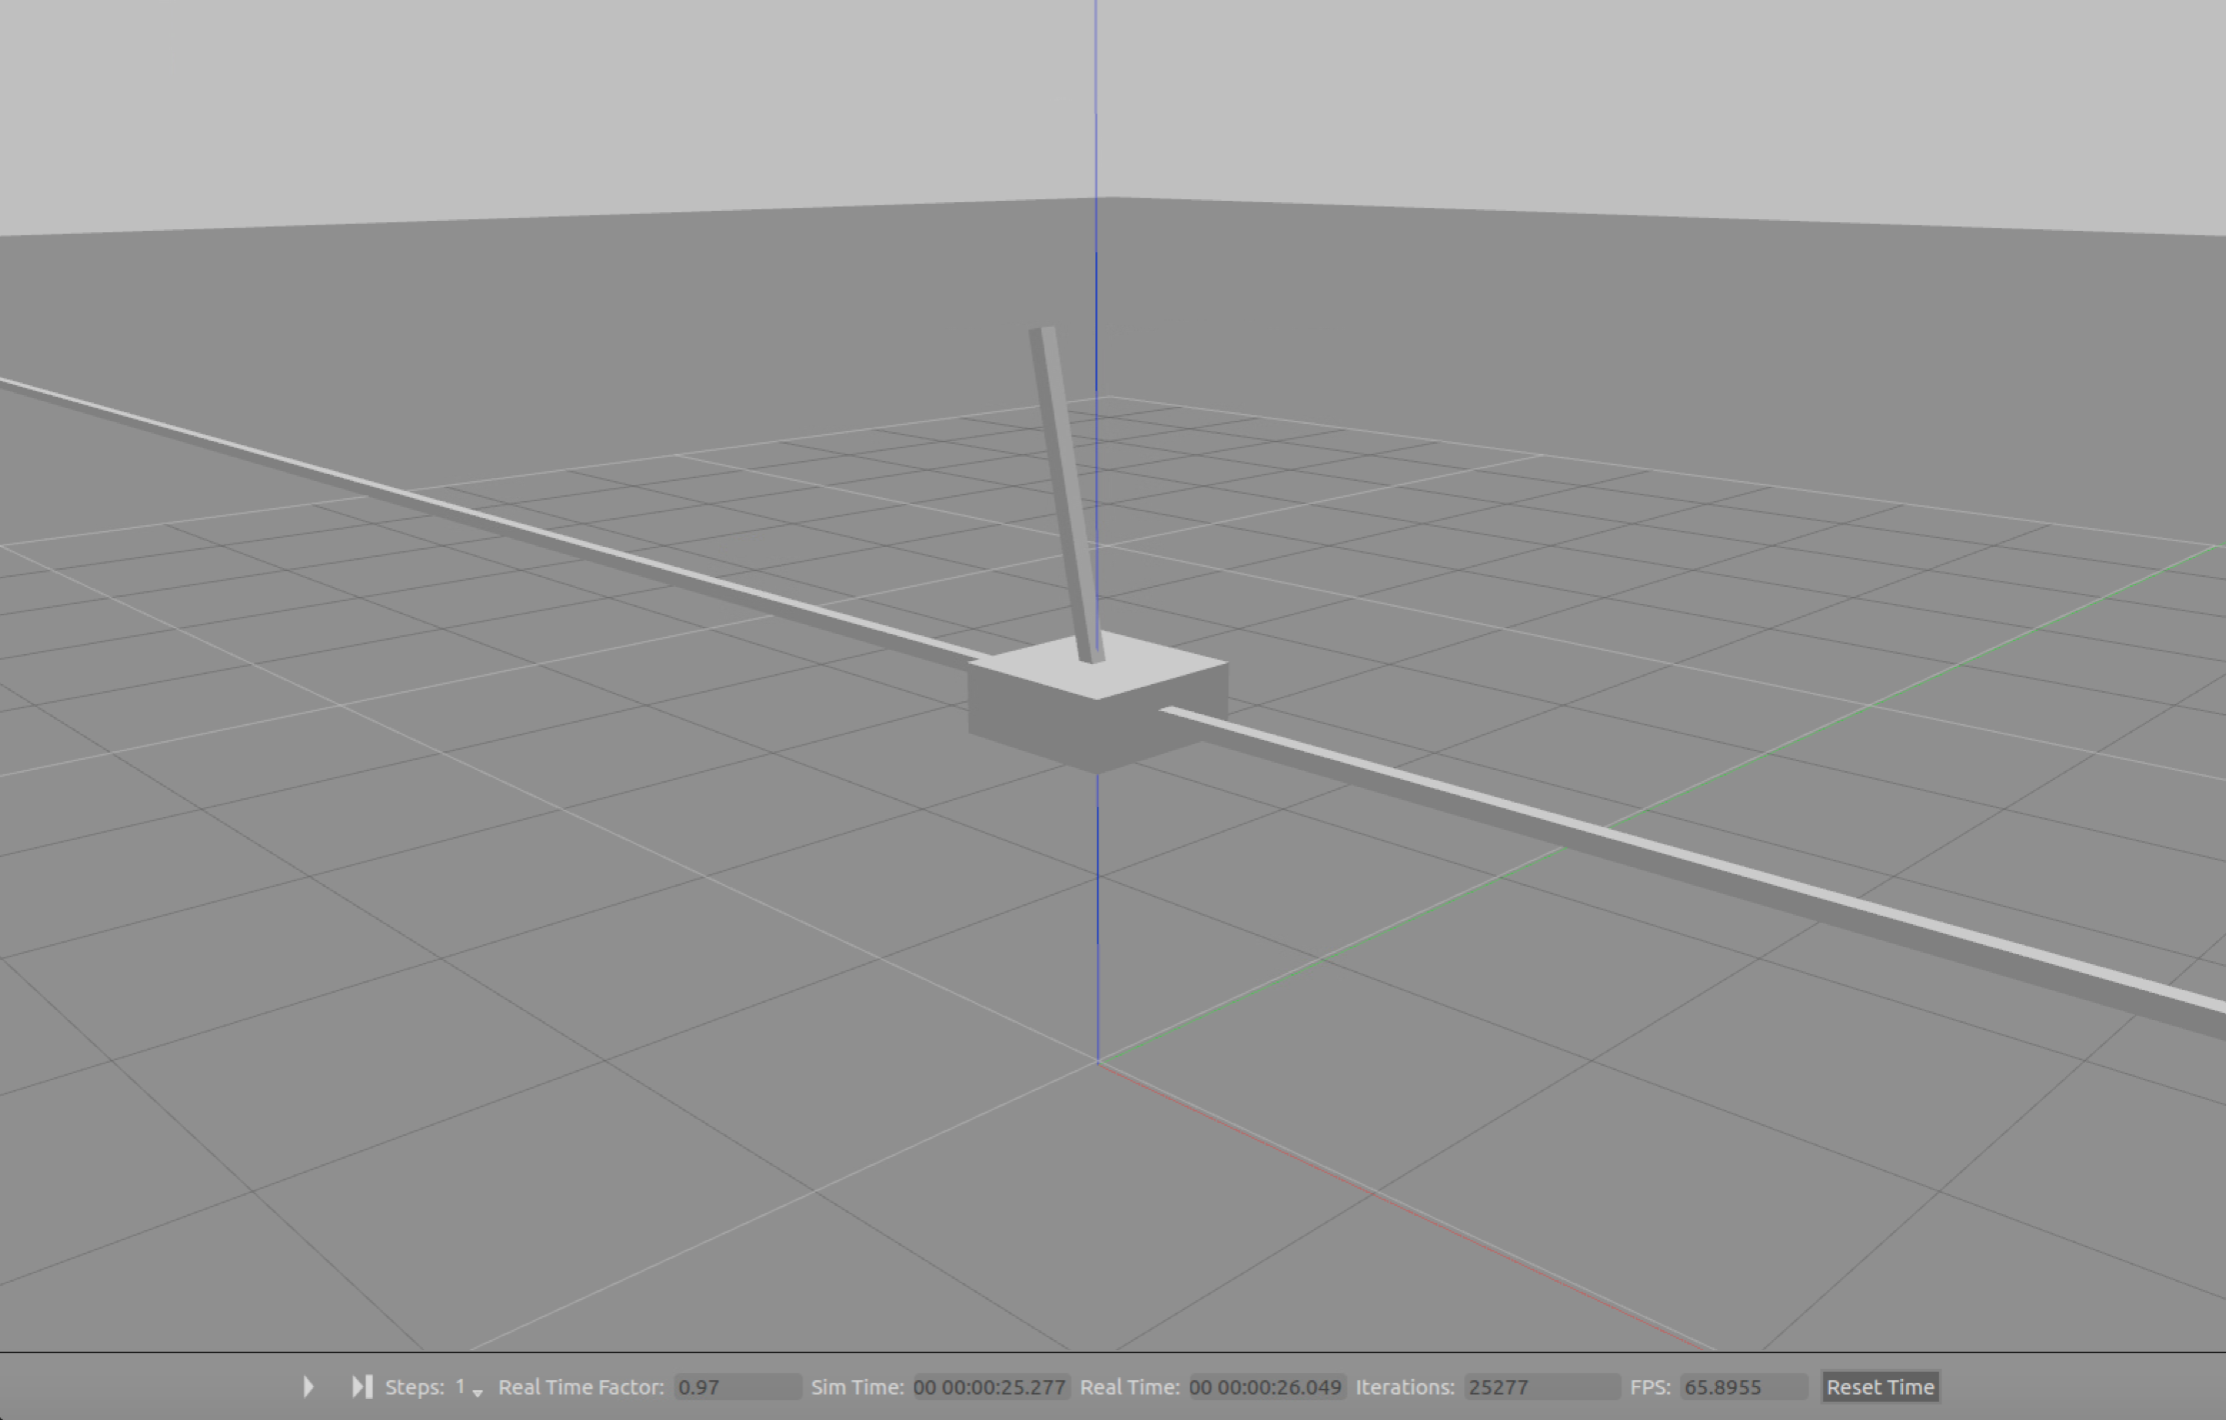
\includegraphics[width=0.8\textwidth]{figs/ch2/cartpole-in-gazebo}
\caption{A Cart-pole model created in Gazebo.}
\label{fig:cartpole-in-gazebo}
\end{figure}

\begin{figure}[h]
\centering
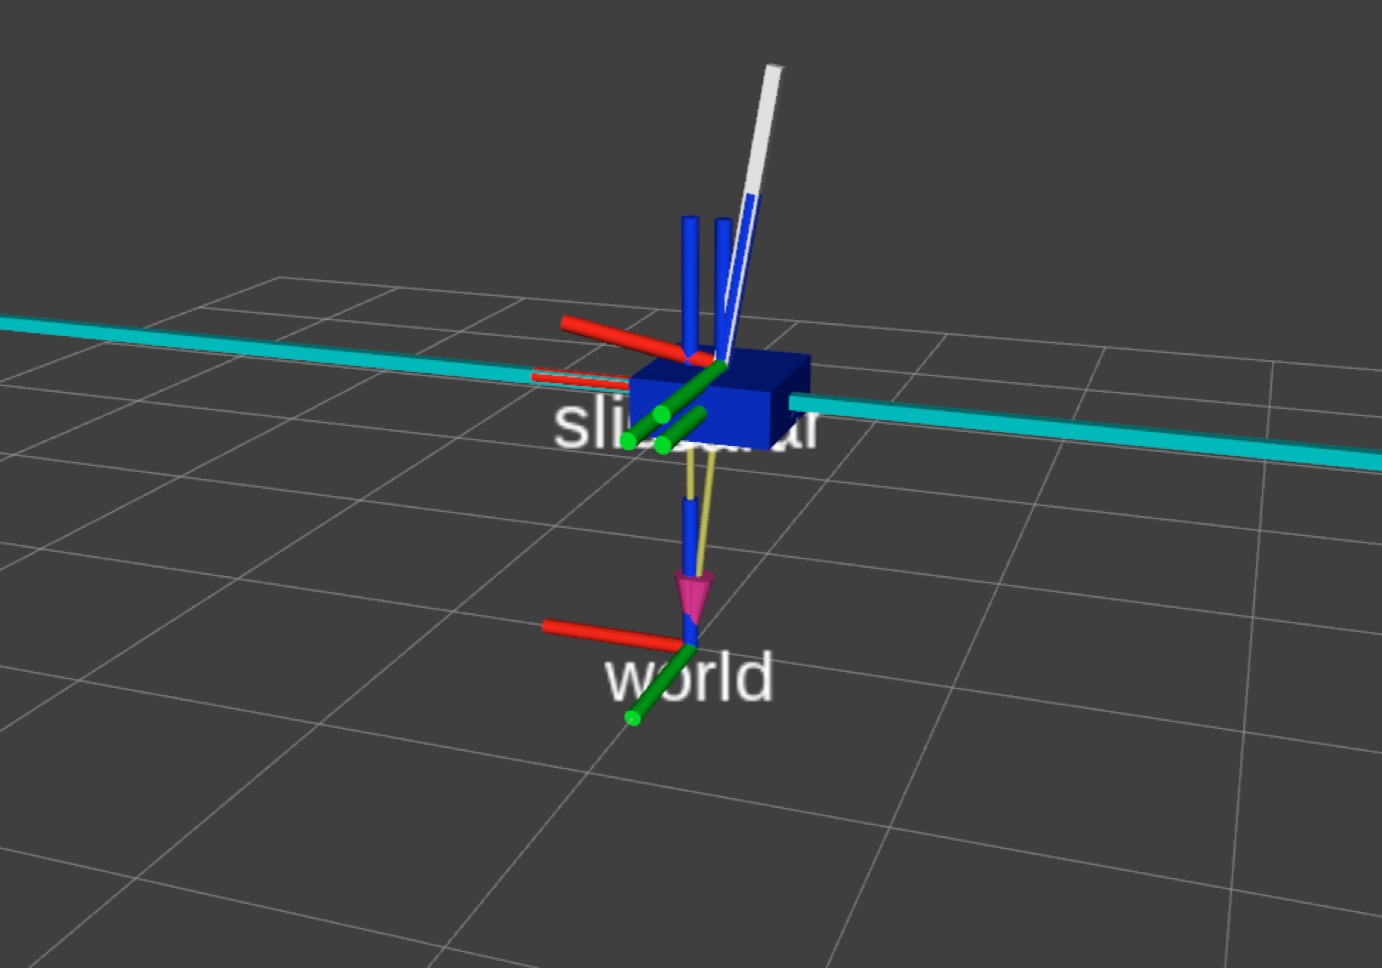
\includegraphics[width=0.8\textwidth]{figs/ch2/cartpole-in-rviz}
\caption{A Cart-pole model displayed in ROS-Rviz.}
\label{fig:cartpole-in-rviz}
\end{figure}

Before we dive into a complex autonomous driving problem on highways, it is helpful to apply the Integrated OpenAI Gym on a simple enough problem, for example, Cart-Pole problem. In this problem or game, the pole needs to keep its balance purely relying on moving the cart in a one-degree axes. A Cart-Pole model was created in Gazebo as shown in Fig. \ref{fig:cartpole-in-gazebo}. The acceptable state follows that the cart is with $\pm 2.4$ meters range and pole is with $\pm 12$ degree angle range. Otherwise, it loses balance and will be initialized to the initial position and angle.

After the controller interface and the \textit{TF} tree are correctly defined, the model and the motion can be monitored in ROS-rviz, as shown in Fig. \ref{fig:cartpole-in-rviz}. 

A Q-Learning Algorithm is applied and the policy are defined as below.

\begin{itemize}
\item \textbf{State Space:} [$pos_{cart}$, $vel_{cart}$, $pos_{pole}$, $vel_{pole}$]

\item \textbf{Action Space:} [$vel_{cart} + 1$, $vel_{cart} - 1$]

\item \textbf{Reward Function:} Each step it gains a 1 point reward until it loses balance and reinitialize.
\end{itemize}

where $pos_{cart}$ is the position along the translation axes, $vel_{cart}$ is the linear velocity, $pos_{pole}$ is the angle of the pole compared to the initial pose,  and $vel_{pole}$ is the angular velocity of the pole.

The Neural Network applied here has one layer with 10 units. The other hyperparameters in the experiment are set as below,

\begin{itemize}
\item{Epochs:} 2000.
\item{Learning Rate in policy gradient:} 0.01.
\item{Learning Rate in value gradient:} 0.1.
\end{itemize}

\begin{figure}[h]
\centering
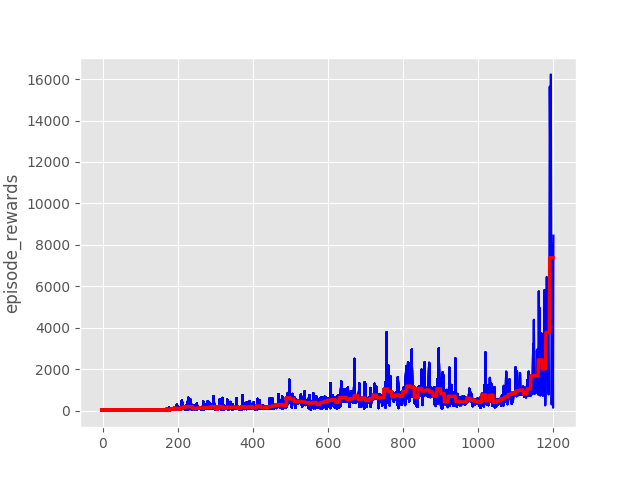
\includegraphics[width=0.8\textwidth]{figs/ch2/cartpole-epoch-1200}
\caption{Reward history of training A Cart-Pole Agent.}
\label{fig:cartpole-result}
\end{figure}

As shown in Fig. \ref{fig:cartpole-result}, the accumulated reward in each episode was gradually increasing and had a huge jump when it came to Episode 1200. After that, it had a satisfying ability to keep balance for a considerable period of time.

%%%%%%%%%%%%%%%%%%%%%%%%%%%%%%%%%%
\section{Vehicle Model}

A well performed vehicle model kit, Dataspeed ADAS Kit Gazebo/ROS Simulator, is adopted here.

\subsection{URDF Models}

\begin{figure}[h]
\centering
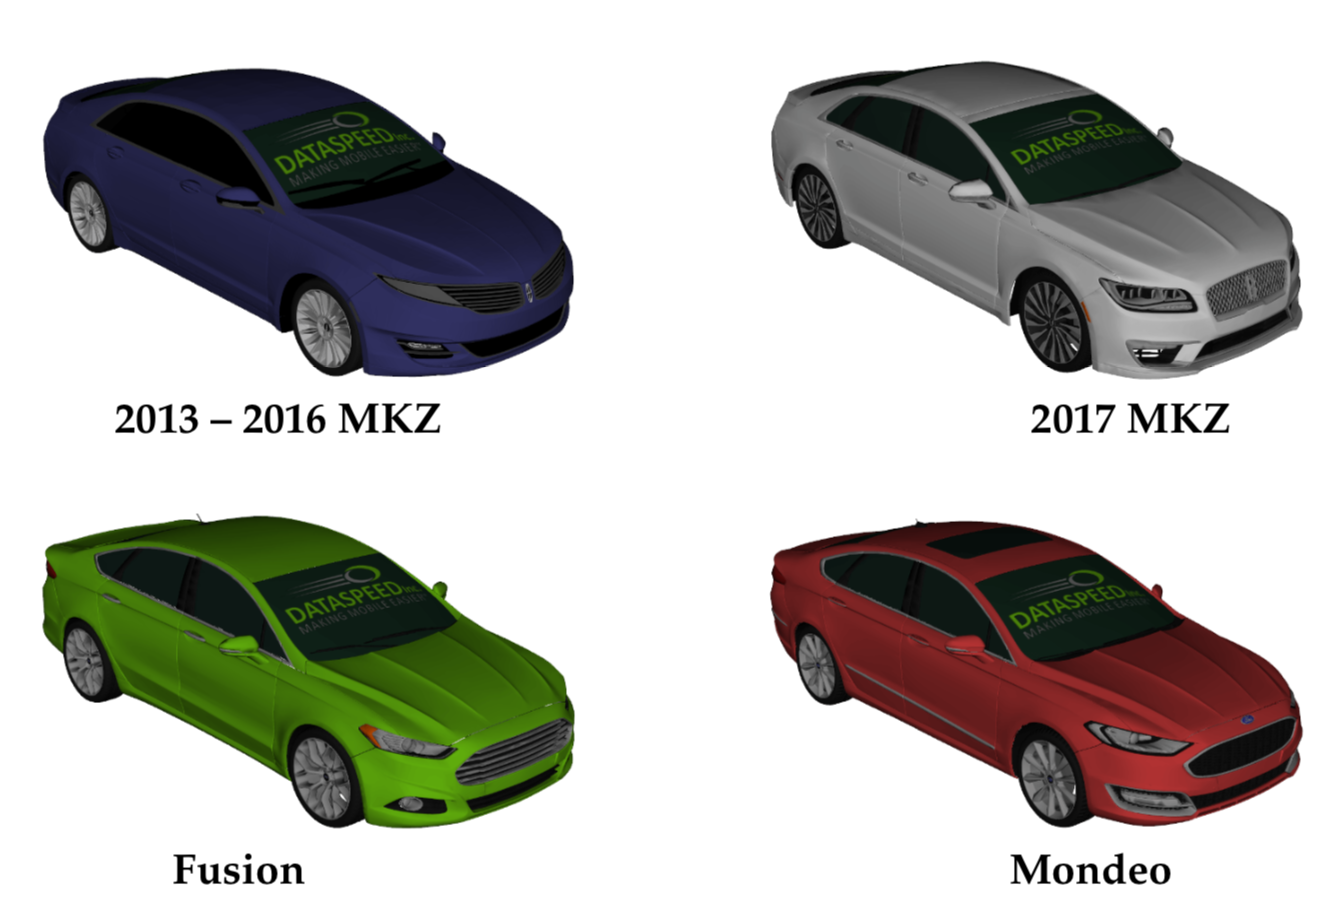
\includegraphics[width=0.8\textwidth]{figs/ch2/mkz-cover}
\caption{4 vehicle models in ADAS Kit.}
\label{mkz-models}.
\end{figure}

Four URDF models representing the different vehicles supported by the Dataspeed ADAS Kit are included in the simulation, as shown in Fig. \ref{mkz-models}. The TF trees of the simulation models are all the same, and this common TF tree is shown in Fig. \ref{fig:dataspeed}.

\begin{figure}
\centering
\begin{minipage}{.5\textwidth}
  \centering
  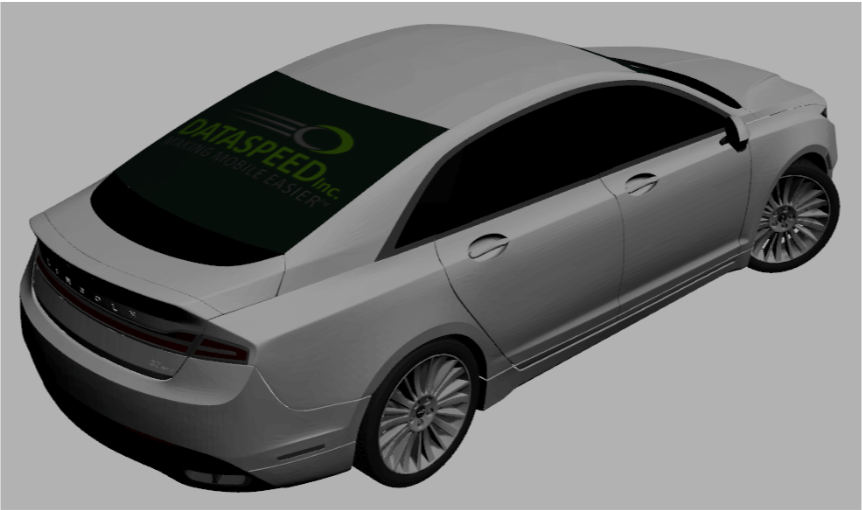
\includegraphics[width=0.9\linewidth]{figs/ch2/mkz-model}
  \label{fig:sub1}
\end{minipage}%
\begin{minipage}{.5\textwidth}
  \centering
  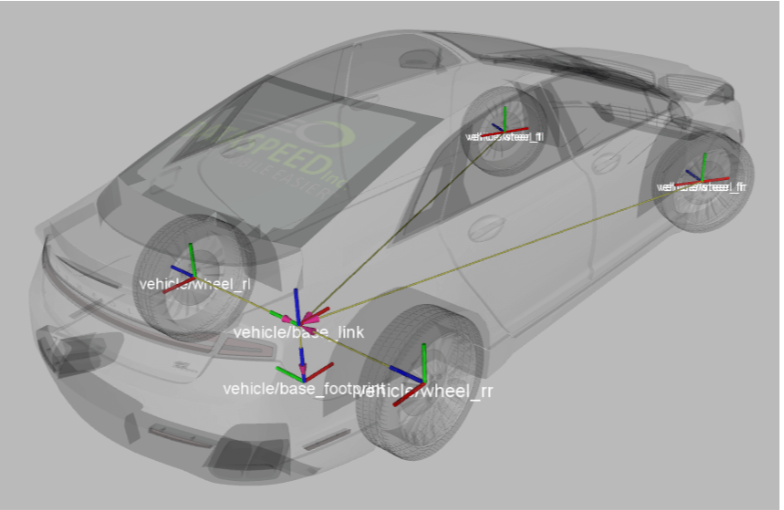
\includegraphics[width=0.82\linewidth]{figs/ch2/mkz-tf-tree}
  \label{fig:sub2}
\end{minipage}
\caption{Simulation model and corresponding TF tree.}
\label{fig:dataspeed}
\end{figure}

\subsection{Simulated CAN Message Interface}

The simulator emulates the CAN message interface to the real ADAS Kit. Therefore, there are only two ROS topics used to interact with the simulated vehicle: $can\_bus\_dbw / can\_tx$ to send CAN messages to the vehicle, and $can\_bus\_dbw / can\_rx$ to receive feedback data from the vehicle. These topics and their corresponding message types are listed in Table \ref{table:dbw1}.

\begin{table}[h!]
\centering
\begin{tabular}{c c} 
 \hline
 Topic Name & Msg Type \\ [0.5ex] 
 \hline
 $~<name>/can\_bus\_dbw/can\_rx$ & $can\_msgs/Frame$  \\ 
 \hline
 $~<name>/can\_bus\_dbw/can\_tx$ & $can\_msgs/Frame$ \\ [1ex] 
 \hline \\
\end{tabular}
\caption{CAN message topics to interact with simulated ADAS Kit.}
\label{table:dbw1}
\end{table}

The simulator only implements a subset of the complete Dataspeed CAN message specification. The supported command messages are listed in Table \ref{table:dbw3}, and the supported report messages are listed in Table \ref{table:dbw3}. See the ADAS Kit datasheets for complete CAN message information.

\begin{table}[h!]
\centering
\begin{tabular}{c c} 
 \hline
 Command Msg & CAN ID \\ [0.5ex] 
 \hline
 Brake & 0x060 \\ 
 \hline
 Throttle &0x062 \\
  \hline
 Steering & 0x064 \\
 \hline
 Gear & 0x066 \\  [1ex] 
 \hline \\
\end{tabular}
\caption{Command CAN messages supported by the ADAS Kit simulator.}
\label{table:dbw2}
\end{table}

\begin{table}[h!]
\centering
\begin{tabular}{c c c} 
 \hline
Report Msg & CAN ID & Data Rate \\ [0.5ex] 
 \hline
Brake & 0x061 & 50 Hz \\
Throttle & 0x063 &  50 Hz \\
Steering & 0x065 & 50 Hz \\
Gear & 0x067 & 20 Hz \\
Misc & 0x069 & 50 Hz \\
Wheel Speed & 0x06A & 100 Hz \\
Accel & 0x06B & 100 Hz \\
Gyro & 0x06C & 100 Hz \\
GPS1 & 0x6D & 1 Hz \\ 
GPS2 & 0x6E & 1 Hz \\
GPS3 & 0x6F & 1 Hz \\
Brake Info & 0x074 & 50 Hz \\ [1ex]
 \hline \\
\end{tabular}
\caption{Report CAN messages supported by the ADAS Kit simulator.}
\label{table:dbw3}
\end{table}


\subsection{Simulating Multiple Vehicles}

The parameters of the ADAS Kit Gazebo simulation are set using a single YAML file. This section describes the options and formatting of the YAML file.

To simulate multiple vehicles simultaneously, simply add more dictionaries to the array in the YAML file. Below is an example:

\begin{lstlisting}[language=XML]
- vehicle1: 
x: -2.0
y: 0.0
color: red
model: mkz
year: 2017

- vehicle2:
x: 0.0
y: 2.0
color: green
model: fusion
\end{lstlisting}

This would spawn two vehicles: one red 2017 MKZ with model name $\textbf{vehicle1}$ spawned at $(0.0, -2.0, 0.0)$ and one green 2013 Fusion with model name $\textbf{vehicle2}$ spawned at $(0.0, 2.0, 0.0)$. Both vehicles would have the default values of the parameters not set in the individual dictionaries.



%\bibliographystyle{plainnat}				%Uncomment this if you want a bibliography on each chapter
%\markright{\textit{Bibliography}}
%\renewcommand{\chaptername}{}
%\bibliography{my_references}

%\vfill

